\documentclass{article}
\usepackage[english]{babel}
\usepackage[utf8]{inputenc}
\usepackage{amsmath,amssymb}
\usepackage{parskip}
\usepackage{graphicx}
\graphicspath{ {./MA2202_images/} }
\newcommand\tab[1][1cm]{\hspace*{#1}}

% Margins
\usepackage[top=2.5cm, left=3cm, right=3cm, bottom=4.0cm]{geometry}


\title{MA2202 (Algebra I)}
\author{Jia Cheng}
\date{September 2021}

\begin{document}

\maketitle

\section{Definitions}
\paragraph{Sets}
\begin{align*}
	\mathbb{N}=\mathbb{Z}^+
\end{align*}
\paragraph{Functions}\mbox{}

Functional equality: 2 functions $f_1:A\rightarrow B, f_2:C\rightarrow D$ are equal iff $A=B\land C=D$ and their elementwise images are equal.

\paragraph{Equivalence Class}\mbox{}
Given a set $S$, an equivalence relation $\equiv$ on $S$. Then the equivalence class of an element $a\in S$ is denoted
\begin{align*}
	Cl(a) = \{x\in S : a\equiv x\}
\end{align*}

\section{Elementary Number Theory}
\paragraph{Coprime cancellation} Suppose $a,b,c$ are non-zero integers and $gcd(a,c)=1$ and $a|bc$.

There are 2 ways to prove $a|b$.

First way, use Bezout's Lemma and multiple $b$ on both sides.\\
Second way actually also uses Bezout's Lemma underlyingly, but we can view it atomically as follows.

\textbf{Lemma} $gcd(a,c)=1$, then there exists an "inverse" $c'$ of $c$ such that $cc'\equiv 1 (\mod a)$.

Since $bc\equiv 0 (\mod a)$, we multiply $c'$ on both sides to get $b\equiv bcc'\equiv 0(\mod a)$. Hence $a|b$.

\paragraph{Fermat's Little Theorem}
Given prime $p$, $a\in \mathbb{Z}$, we have 
\begin{align*}
	a^p \equiv a (\mod p)
\end{align*}

If $p$ does not divide $a$, then we use cancellation to get $a^{p-1}\equiv 1(\mod p)$

\paragraph{Chinese Remainder Theorem} Taken from Brilliant

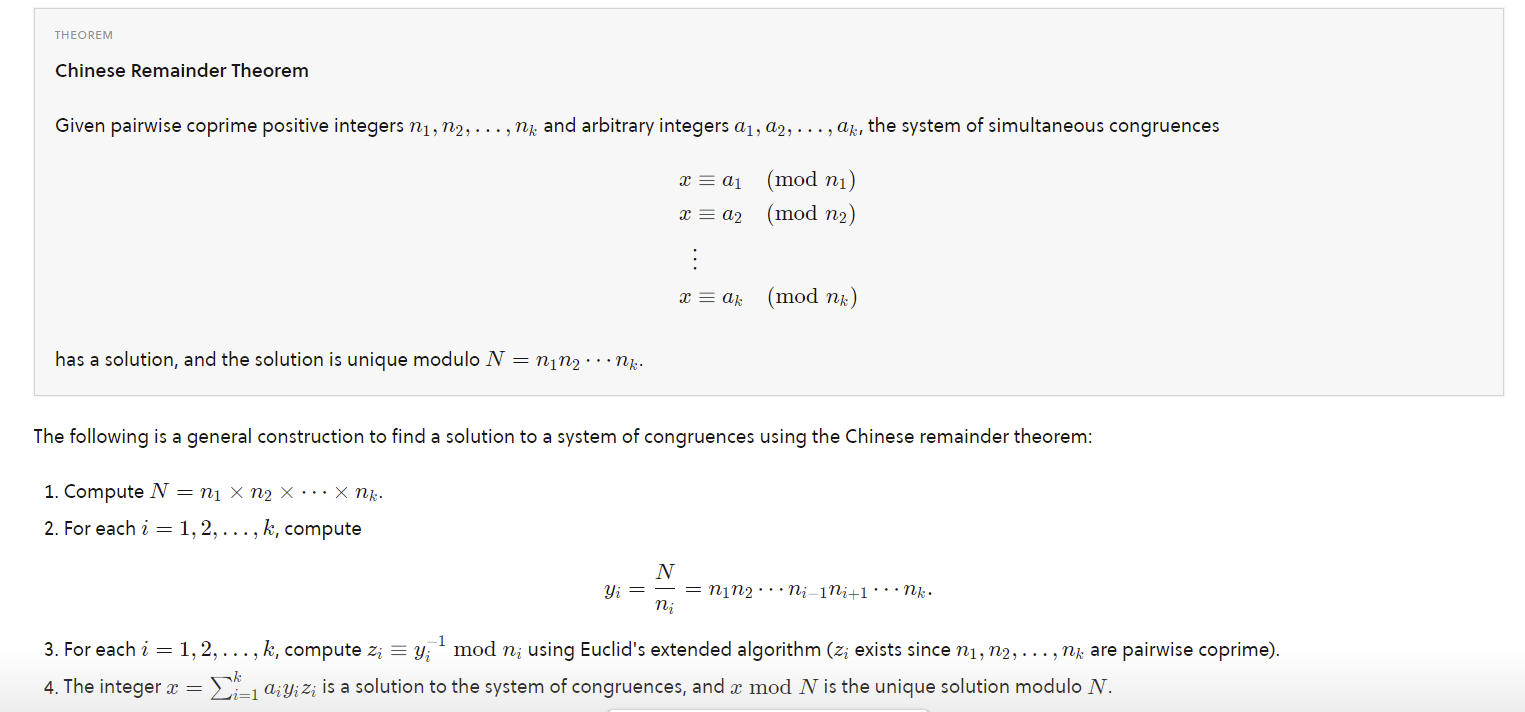
\includegraphics[scale=0.55]{ChineseRemainderTheorem}


\section{Groups}
\paragraph{Group axioms}
\begin{itemize}
	\item When proving axiom G4, closure under inverses, to show that $y$ is an inverse of $x\in G$, \textbf{we need to show that} $y\in G$ in addition to showing that $xy=yx=e$. Too frequently the detail that $y\in G$ is not explicitly proven.
	\item This also applies if we want to prove a certain element is the identity. We may need to prove that the element lies in $G$ first.
\end{itemize}

\section{Counterexamples}
\paragraph{Operations}\mbox{}
Commutative but not associative
\begin{itemize}
	\item Taking arithmetic mean/geometric mean of 2 numbers
	\item Taking the difference of 2 numbers $|a-b|$
\end{itemize}

Associative but not commutative
\begin{itemize}
	\item Function composition
	\item Matrix multiplication
	\item $(x,y)\mapsto y$
\end{itemize}

\section{Symmetric groups}
\paragraph{Isomorphism between 2 permutation groups}
Let $S_n$ be the symmetric group of order $n$, and $S_Y$ be the permutation group on $Y$, where $|Y|=n$. We write $Y=\{x_1,\dots, x_n\}$\\
Then there are 2 ways in which we can define an isomorphism $\phi:S_n\rightarrow S_Y$.

First, a more indirect definition. Let $f:\{1,2,\dots, n\}\rightarrow \{1,2,\dots, n\}$. Then $f\in S_n$. Define $\phi(f)$ as the mapping 
\begin{align*}
	\phi(f): x_i \mapsto x_{f(i)}
\end{align*}
It is then easy to prove the homomorphic properties of $\phi$. $\phi(f\circ g)(x_i) = x_{(f\circ g)(i)} = x_{f(g(i))} = (\phi(f)\circ \phi(g))(x_i)$.

Second, we define the mapping $T: i\rightarrow x_i$ and consequently, $\phi = T\circ f\circ T^{-1}$.\\
Then $\phi(f\circ g) = T\circ f\circ g\circ T^{-1} = T\circ f\circ T^{-1}\circ T\circ g\circ T^{-1}$.

\paragraph{Cyclic notations}\mbox{}
Given 2 products $A, B$ of disjoint permutation cycles, themselves also being pairwise disjoint. There are permutations $f,g$ such that $A$ represents $f$ and $B$ represents $g$.
Now we want to prove the following properties.

\begin{itemize}
	\item $AB$ represents $f\circ g$. Proving this would allow us to make use of the properties of functional composition to claim that $A(BC)=(AB)C$, where $A,B,C$ are products of disjoint permutation cycles. (and $A,B,C$ are themselves pariwise disjoint).\\
	To prove this we consider cases: whether $x$ lies in the cycles of $A$, whether $x$ lies in the cycles of $B$, or neither. Note that if $x$ does not lie in the cycles of $A$ for e.g., then $f(x)=x$.
	\item $AB=BA$. To show this we only need to consider 3 cases. Whether $x$ lies in the cycles of $A$, whether $x$ lies in the cycles of $B$, or neither.
\end{itemize}

\paragraph{Showing equivalence of 2 cycles}

Suppose $c, d$ are 2 cycles such that $\exists i, \forall n\in \mathbb{N}, c^n(i) = d^n(i)$, where for a function $f$, $f^n$ denotes composition $n$ times.

We first write out $c = (i, c(i), \dots, c^{|c|-1}(i))$

Then in particular $\forall n\in \{0, 1\dots, |c|-1\}, c^n(i) = d^n(i)$, $d^n(i) = c^n(i)$ and $d^{|c|}(i) = c^{|c|}(i) = i$, which says that $d = (i, c(i), \dots, c^{|c|-1}(i))$. Hence $d=c$.

Notice that the key part of this argument is to show that $d$ loops around, i.e. $d(c^{|c|-1}(i)) = i$.

\end{document}


